\subsection{Анализ функции}

\subsubsection{Седловые точки}

Рассмотрим функцию двух переменных:
\[
  f(x,y)=10^{-2}(8x^2+2xy+43x+10y+15)
\]

Это квадратичная функция, которая определена в заданной области \( \mathcal{D} \). Исследуем её на наличие \textit{седловых точек} --- стационарных точек, которые не являются точками экстремума.

По необходимому условию экстремума второго порядка для точки \( (x,y) \):
\[
  \begin{cases}
    \frac{\partial f}{\partial x}(x,y)=0\\
    \frac{\partial f}{\partial y}(x,y)=0
  \end{cases}
  \implies
  \begin{cases}
    10^{-2}(16x + 2y + 43) = 0 \\
    10^{-2}(2x + 10) = 0
  \end{cases}
  \implies
  \begin{cases}
    x = -5 \\
    y = 18.5
  \end{cases}
\]

Точка \( M=(-5,18.5)\in\mathcal{D} \), поэтому продолжим её исследование. Для проверки достаточного условия найдём матрицу Гессе:
\[
  H=\begin{pmatrix}
    \frac{\partial^2 f}{\partial x^2}(x,y) & \frac{\partial^2 f}{\partial x\partial y}(x,y)\\
    \frac{\partial^2 f}{\partial y\partial x}(x,y) & \frac{\partial^2 f}{\partial y^2}(x,y)\\
  \end{pmatrix}=10^{-2}\cdot\begin{pmatrix}
    16 & 2\\
    2 & 0
  \end{pmatrix}
\]

Заметим, что определитель постоянный для \( M \). Имеем ситуацию:
\[
  \Delta_1=16\cdot 10^{-2}\quad\Delta_2=-4\cdot 10^{-4}
\]

Поскольку \( \Delta_2<0 \), то точка \( M \) не является точкой экстремума. Это значит, что она \textit{седловая по определению}. Для полноты описания приведём значение функции в данной точке:
\[
  f(M)=0
\]

\subsubsection{Глобальный минимум}

Функция рассматривается в области \( \mathcal{D} \), которая является компактом \textit{(оно замкнуто и ограничено)}. Поскольку \( f\in C(\mathcal{D}) \), по теореме Вейерштрасса о функции на компакте \( f \) достигает своего наименьшего значения.

Как выяснилось в предыдущем разделе, у функции нет точек экстремума в области \( \mathcal{D} \). Поэтому исследуем границы области и найдём глобальный минимум:

\begin{enumerate}
  \item Точка лежит на \textit{левой} стороне прямоугольника (\( x=-20, y \in [-50, 50] \)):
  \[
    f_1(y) = 10^{-2}(2355 - 30y)
  \]
  Функция \( f_1 \) линейна относительно \( y \). Она убывает, поэтому минимум достигается в точке \( y=50 \):
  \[
    f_1(50) = 10^{-2}(2355 - 1500) = 8.55
  \]
  \item Точка лежит на \textit{правой} стороне квадрата (\( x=20,y\in[-50,50] \)):
  \[
    f_2(y) = 10^{-2}(4075 + 50y)
  \]
  Функция \( f_2 \) линейна относительно \( y \). Она возрастает, поэтому минимум достигается в точке \( y=-50 \):
  \[
    f_2(-50) = 10^{-2}(4075 - 2500) = 15.75
  \]
  \item Точка лежит на \textit{верхней} стороне квадрата (\( x=\in[-20,20],y=50 \)):
  \[
    f_3(x) = 10^{-2}(8x^2 + 143x + 515)
  \]
  Это квадратичная функция, у которой ветви направлены вверх, так как \( 8\cdot 10^{-2}>0 \). Следовательно, минимум лежит на вершине параболы:
  \[
    x_{\text{в}}=-\dfrac{143}{16}\in[-20,20]\implies f_3(x_{\text{в}})= -1.2403125
  \]
  \item Точка лежит на \textit{нижней} стороне прямоугольника (\( x \in [-20, 20], y=-50 \)):
  \[
    f_4(x) = 10^{-2}(8x^2 - 57x - 485)
  \]
  Это квадратичная функция, у которой ветви направлены вверх, так как \( 8\cdot 10^{-2}>0 \). Следовательно, минимум лежит на вершине параболы:
  \[
    x_{\text{в}} = \dfrac{57}{16}\in[-20,20] \implies f_4(x_{\text{в}})= -5.8653125
  \]
\end{enumerate}

После рассмотрения границ можно сделать вывод, что на нижней стороне области \( \mathcal{D} \) лежит глобальный минимум области:
\[
  \arg\min_{(x,y)\in\mathcal{D}}f(x,y)=\left(\dfrac{57}{16},-50\right)\implies f\left(\dfrac{57}{16},-50\right)= -5.8653125
\]

\subsubsection{Линии уровня}

Ниже изображены линии уровня данной по варианту функции \( f(x) \). Белым отмечена найденная седловая точка \( M \) в области \( \mathcal{D} \), а красным --- точка глобального минимума.

\begin{figure}[H]
  \centering
  \begin{adjustbox}{max width=.9\textwidth,keepaspectratio}
    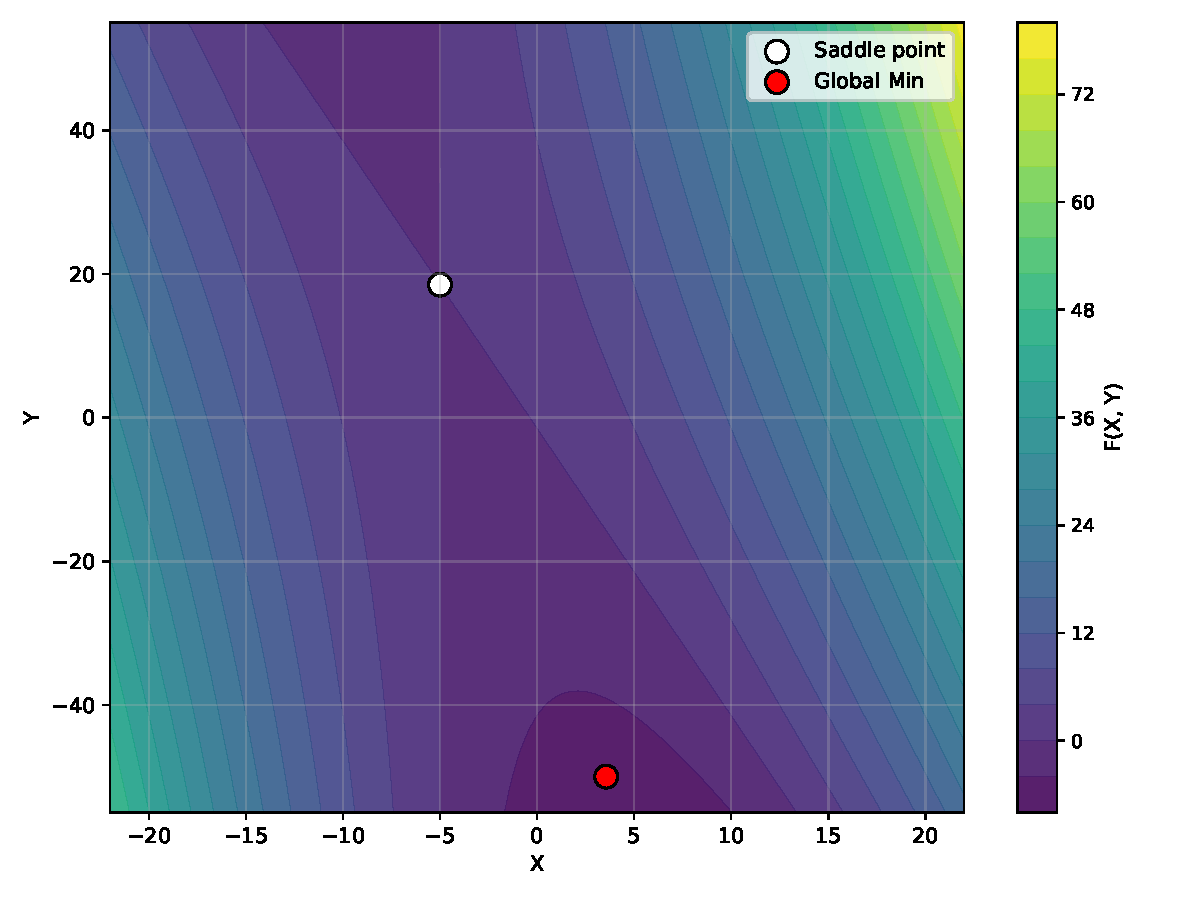
\includegraphics{pics/contour_lines.pdf}
  \end{adjustbox}
  \caption{Линии уровня \( f(x) \) с седловой точкой \( M \).}
\end{figure}

\subsubsection{Потенциальные сложности оптимизации}

Если воспользоваться численными методами первого порядка для оптимизации \( f(x) \) в области \( \mathcal{D} \), то могут возникнуть следующие трудности:

\begin{itemize}
  \item Поверхность имеет ярко выраженный «овражный» характер. Значит, градиентный спуск может совершать резкие поперечные колебания (\textit{пилообразное движение}), что замедляет поиск решения.
  \item Слишком малая скорость обучения сделает движение вдоль пологого «дна» оврага чрезвычайно медленным, что потребует огромного числа итераций.
  \item Классический градиентный спуск может застрять в окрестности седловой точки, так как градиент \( \nabla f\approx 0 \).
  \item В зависимости от начального приближения алгоритм может сойтись к~локальному минимуму на другой стороне прямоугольника.
\end{itemize}